\section{Auswertung}
\label{sec:Auswertung}

\subsection{Überprüfung der Bragg-Bedingung}

Bei einem Kristallwinkel von 14° ergibt sich die folgende Intensitätsverteilung
hinter dem LiF-Kristall, an dem die Bragg-Reflexion stattgefunden hat.

\begin{figure}
  \centering
  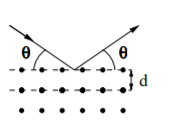
\includegraphics{bragg.pdf}
  \caption{Intensität in Abhängigkeit des Winkels bei Bragg-Reflexion.}
  \label{fig:bragg}
\end{figure}

Das Maximum liegt bei ca. 27,7°. Erwartet wurde das Maximum entsprechend der
Bragg-Bedingung (Gleichung 6) bei einem Winkel von 28°. Der gemessene Wert weicht
also lediglich um etwa 0,3° ab.


\subsection{Emissionsspektrum der Kupferröntgenröhre}

Die Intensität $I$ der gemessenen Röntgenstrahlung wird gegen den doppelten Winkel $\Theta$ des Zählrohrs aufgetragen.

\begin{figure}[H]
  \centering
  \includegraphics{plot.pdf}
  \caption{Emissionsspektrum der Kupferröntgenröhre.}
  \label{fig:plot}
\end{figure}

Der erste sichtbare Peak ist die $K_{\beta}$-Linie und der zweite peak die $K_{\alpha}$-Linie.
Der Grenzwinkel beträgt $8$°.
Mit Gleichung (1) folgt für die maximale Energie:
\begin{equation}
  E = \frac{hc}{2d \sin{\Theta}} = 22,2 \symup{keV}
\end{equation}

Der zu erwartende Wert wäre $35$keV gewesen.
Dies entspricht einer Abweichung von $36,6 \%$.

Das Maximum der $K_{\beta}$-Linie beträgt $I=1624$.

Die Maxima des Spektrums liegen bei den Winkeln $\Theta_{\beta} = 20,2°$ und $\Theta_{\alpha} = 22,2°$.
Mit Gleichung (7) folgt daraus für die Energien:
\begin{align*}
  E_{\beta} &= 8,93 \symup{keV} \\
  E_{\alpha} &= 8,16 \symup{keV}
\end{align*}

Mit Gleichung (3) werden daraus die beiden Abschirmzahlen $\sigma_1$ und $\sigma_2$ berechnet.
\begin{align*}
  \sigma_1 &= Z - \sqrt{\frac{E_{\beta}}{R_{\infty}}} = 3,38 \\
  \sigma_2 &= Z - \sqrt{4 \frac{R_{\infty} (Z-\sigma_1)^2 - E_{\alpha}}{R_{\infty}}} = 13,98
\end{align*}

Zur Bestimmung der Halbwertsbreite wird der Bereich um die $K^{\alpha}$ und $K^{\beta}$ Strahlung
noch einmal genau aufgetragen.

\begin{figure}
  \centering
  \includegraphics{plot1.pdf}
  \caption{Emissionsspektrum der Kupferröntgenröhre im Bereich der charakteristischen Strahlung.}
  \label{fig:plot1}
\end{figure}

Die Winkel der Halbwertsbreiten betragen:
\begin{align*}
  \Theta_{\beta_1} = 19,9° \\
  \Theta_{\beta_2} = 20,4° \\
  \Theta_{\alpha_1} = 22,1° \\
  \Theta_{\alpha_2} = 22,6° \\
\end{align*}
Daraus ergeben sich dich Halbwertsbreiten:
\begin{equation*}
  b_{\alpha} = 0.59°
\end{equation*}

\begin{equation*}
  b_{\beta} = 0.44°
\end{equation*}



Für die Energiedifferenz $\Delta E_{\beta} = E_{\Theta_1} - E_{\Theta_2}$ der $K_{\beta}$-Linie ergibt sich durch Gleichung (7):
\begin{align*}
  \Delta E_{\beta} =  (9,07 - 8,86) \symup{keV} = 0,21 \symup{keV}
\end{align*}

Für die Energiedifferenz $\Delta E_{\alpha} = E_{\Theta_1} - E_{\Theta_2}$ der $K_{\beta}$-Linie ergibt sich durch Gleichung (7):
\begin{align*}
  \Delta E_{\alpha} =  (8,21 - 8,04) \symup{keV} = 0,17 \symup{keV}
\end{align*}

\subsection{Absorptionsspektrum von Brom}

Die Intensität der gemessenen Röntgenstrahlung wird in Abhängigkeit von dem doppelten Zählrohrwinkel für
einen Bromabsorber aufgetragen.

\begin{figure}[H]
  \centering
  \includegraphics{plotbrom.pdf}
  \caption{Absorptionsspektrum von Brom.}
  \label{fig:plot}
\end{figure}

Das Maximum der Intensität liegt bei einem Winkel von $\Theta_{Br} = 13,4°$.
Mit Gleichung (7) beträgt die Energie:
\begin{align*}
  E_{Br} = 13,31 \symup{keV}
\end{align*}
Der Literaturwert beträgt $E_{lit} = 13,48 \symup{keV}$ und die relative Abweichung $-1,3\%$.

Mit Gleichung (3) wird daraus die Abschirmzahl $\sigma_{Br}$  berechnet.

\begin{align*}
  \sigma_1 &= Z - \sqrt{\frac{E_{Br}}{R_{\infty}}} = 3,52 \\
\end{align*}

Der Literaturwert beträgt $\sigma_{lit} = 3,51$ und die relative Abweichung $0,28\%$.

\subsection{Absorptionsspektrum von Strontium}

Die Intensität der gemessenen Röntgenstrahlung wird in Abhängigkeit von dem doppelten Zählrohrwinkel für
einen Strontiumabsorber aufgetragen.

\begin{figure}[H]
  \centering
  \includegraphics{plotstrontium.pdf}
  \caption{Absorptionsspektrum von Strontium.}
  \label{fig:plot}
\end{figure}

Das Maximum der Intensität liegt bei einem Winkel von $\Theta_{Sr} = 11,2°$.
Mit Gleichung (7) beträgt die Energie:

\begin{align*}
  E_{Sr} = 15,88 \symup{keV}
\end{align*}

Der Literaturwert beträgt $E_{lit} = 16,10 \symup{keV}$ und die relative Abweichung $-1,4\%$.


Mit Gleichung (3) wird daraus die Abschirmzahl $\sigma_{Sr}$  berechnet.

\begin{align*}
  \sigma_1 &= Z - \sqrt{\frac{E_{Sr}}{R_{\infty}}} = 3,83 \\
\end{align*}

Der Literaturwert beträgt $\sigma_{lit} = 3,59$ und die relative Abweichung $6,69\%$.


\subsection{Absorptionsspektrum von Zirconium}

Die Intensität der gemessenen Röntgenstrahlung wird in Abhängigkeit von dem doppelten Zählrohrwinkel für
einen Zirconiumbsorber aufgetragen.

\begin{figure}[H]
  \centering
  \includegraphics{plotzirconium.pdf}
  \caption{Absorptionsspektrum von Zirconium.}
  \label{fig:plot}
\end{figure}


Das Maximum der Intensität liegt bei einem Winkel von $\Theta_{Zr} = 10,1°$.
Mit Gleichung (7) beträgt die Energie:
\begin{align*}
  E_{Zr} = 17,59 \symup{keV}
\end{align*}

Der Literaturwert beträgt $E_{lit} = 18,00 \symup{keV}$ und die relative Abweichung $-2,3\%$.

Mit Gleichung (3) wird daraus die Abschirmzahl $\sigma_{Zr}$  berechnet.

\begin{align*}
  \sigma_1 &= Z - \sqrt{\frac{E_{Zr}}{R_{\infty}}} = 4,04 \\
\end{align*}

Der Literaturwert beträgt $\sigma_{lit} = 3,62$ und die relative Abweichung $11,6\%$.


\subsection{Bestimmung der Rydberg-Energie}

Die Wurzel der Absorptionsenergie wird gegen die Ordnungszahl der drei Absorber aufgetragen.

\begin{figure}[H]
  \centering
  \includegraphics{plotmoseley.pdf}
  \caption{Absorptionsenergien in Abhängigkeit von der Ordnungszahl der Elemente.}
  \label{fig:plot}
\end{figure}

Die lineare Regression, sowie die Berechnung der Steigung $a$ und dessen Fehler wird mit Python durchgeführt.
Die Steigung beträgt:
\begin{align*}
  a = \SI{0.10451(1)}{\sqrt{\kilo\eV}}
\end{align*}

Für die Rydberg-Energie in eV gilt dann:
\begin{align*}
  R_{\infty} = \frac{a^2}{1000} =\SI{10.922(2)}{\eV}
\end{align*}

Die relative Abweichung zum Literaturwert beträgt $-19,7 \%$.


\subsection{Absorptionsspektrum von Quecksilber}

Die Intensität der gemessenen Röntgenstrahlung wird in Abhängigkeit von dem doppelten Zählrohrwinkel für
einen Zirconiumbsorber aufgetragen.

\begin{figure}[H]
  \centering
  \includegraphics{plotquecksilber.pdf}
  \caption{Absorptionsspektrum von Quecksilber.}
  \label{fig:plot}
\end{figure}


Die Maxima der Intensität liegen bei einem Winkel von $\Theta_{L1} = 19,9°$  und $\Theta_{L2} = 20,25°$.
Mit Gleichung (7) beträgt die Energie:
\begin{align*}
  E_{Hg,1} = 9,06 \symup{keV} \\
  E_{Hg,2} = 8,91 \symup{keV}
\end{align*}

Mit Gleichung (5) wird daraus die Abschirmkonstante $\sigma_{L, Hg}$ berechnet.
\begin{equation*}
  \sigma_{L, Hg} = 78,58
\end{equation*}
